\documentclass[11pt]{article}

\usepackage[margin=1in]{geometry}
\usepackage{amsmath,amssymb,amsfonts}
\usepackage{booktabs,longtable,array,multirow}
\usepackage{graphicx}
\usepackage{xcolor}
\usepackage{hyperref}
\usepackage{enumitem}
\usepackage{tikz}
\usetikzlibrary{positioning}
\usepackage{pgfplots}
\usepackage{tcolorbox}
\usepackage{natbib}
\usepackage{listings}
\usepackage{caption}
\usepackage{subcaption}
\usepackage{microtype}
\pgfplotsset{compat=1.18}

\hypersetup{
  colorlinks=true,
  linkcolor=blue!55!black,
  citecolor=blue!55!black,
  urlcolor=blue!55!black
}

\definecolor{mmalsblue}{RGB}{0,80,130}
\definecolor{mmalsgreen}{RGB}{32,110,80}
\definecolor{mmalsamber}{RGB}{180,105,20}
\definecolor{mmalsgray}{RGB}{80,80,80}
\definecolor{storybg}{RGB}{246,250,248}
\definecolor{riskbg}{RGB}{255,248,240}

\newtcolorbox{kidbox}{
  colback=storybg,
  colframe=mmalsgreen!70!black,
  title={Story for a 12-year-old},
  fonttitle=\bfseries,
  arc=2mm,
  boxrule=0.8pt
}

\newtcolorbox{claimbox}{
  colback=riskbg,
  colframe=mmalsamber!80!black,
  title={Claim status},
  fonttitle=\bfseries,
  arc=2mm,
  boxrule=0.8pt
}

\newcommand{\mmals}{\textsc{MMALS}}
\newcommand{\rc}{\textsc{RC}}
\newcommand{\zf}{z_f}
\newcommand{\Dr}{D_r}
\newcommand{\Dz}{D_z}
\newcommand{\Dy}{D_y}

\title{\Large Mycelium-Inspired Mutualistic Adaptive Learning Systems (\mmals):\\
A Research Chronicle from Bio-Inspired Functional Memory to Auditable Inferred-Context Continual Learning}
\author{Guillaume Harbonnier\\\small Draft research article and reproducibility package}
\date{Compiled May 2026}

\begin{document}
\maketitle

\begin{abstract}
This paper consolidates the research trajectory of Mycelium-Inspired Mutualistic Adaptive Learning Systems (\mmals), a bio-inspired continual-learning program that treats memory not as a static parameter snapshot but as a mediated functional exchange across specialists. The project began as a mycelium metaphor for routing and mutualistic exchange, then progressively became an experimental continual-learning harness with explicit baselines, functional drift diagnostics, inferred context, no-leakage policy selection, and audit artifacts. The central thesis that emerged is that the relevant memory object is not merely the selected route, but the function computed through that route: routes, latent transformations, outputs, context posteriors, and readout policies must be observed together. We review the sequence from v0.1 to v1.1-RC2H, including route-function disentanglement, comparative benchmarks, Hopfield and co-evolution controls, geometry and fluid-inspired diagnostics, inferred-context stress, and the recent RC2 selector lineage. Evidence to date supports the value of functional-memory diagnostics and guarded context-sensitive deployment policies, but does not yet justify production-readiness claims. The latest evidence identifies a stable deployable anchor family, while showing that free validation-based policy selection can still underperform. The next milestone is multi-dataset robust qualification across MNIST, FashionMNIST, RotatedMNIST, and PermutedMNIST, followed by v0.11-style comparative benchmarking with accuracy, forgetting, cost, memory, parameters, runtime, and auditability.
\end{abstract}

\begin{claimbox}
This is a research article and packaging draft, not a peer-reviewed paper and not a production certification. The strongest current claim is: \emph{\mmals has a promising, auditable inferred-context continual-learning mechanism with replay-beating evidence on FashionMNIST overlap-chain tests, but the automatic selector is not yet sufficiently reliable to replace safe anchored policies.}
\end{claimbox}

\tableofcontents
\newpage

\section{Executive summary}

The story of \mmals is the story of a metaphor becoming a measurement program. The early metaphor was biological: a fungal medium connects several hosts, routes energy, exchanges nutrients, and preserves useful adaptations. The machine-learning translation became a continual-learning system with several specialist hosts, transformations, a routing matrix, a mediated latent state, and memory losses that preserve old behavior while learning new tasks.

The research program evolved through four major scientific transitions.

\begin{enumerate}[label=\textbf{T\arabic*.},leftmargin=*]
  \item \textbf{From route memory to functional memory.} Early versions asked whether preserving the route was enough. The answer became no: the same route can compute a different function if hosts or transformations drift.
  \item \textbf{From explicit task IDs to inferred context.} Early versions knew the task. The v1 direction asks whether the model can infer the situation from the input and memory.
  \item \textbf{From performance-only notebooks to evidence harnesses.} v0.11 and later introduced baselines, cost, parameters, runtime, forgetting, and reproducibility artifacts.
  \item \textbf{From free selection to conservative deployment.} RC2b-RC2H showed that selecting a policy only by validation proxy can choose fragile policies. The next selector must be anchored on safe guarded policies and allow overrides only with strong evidence.
\end{enumerate}

\begin{kidbox}
Imagine a forest where different trees are good at different things. A mushroom network connects them. At first we asked: ``Did the mushroom use the same path as before?'' Later we learned that this is not enough. The path can be the same, but the message carried along the path can change. So the real question became: ``Did the forest still solve the old problem in the same useful way while learning a new problem?''
\end{kidbox}

\section{Scientific motivation}

Continual learning studies how a model can learn a sequence of tasks without catastrophically forgetting earlier tasks. Classical approaches include regularization methods such as Elastic Weight Consolidation \citep{kirkpatrick2017ewc}, distillation-based methods such as Learning without Forgetting \citep{li2017lwf}, replay methods, progressive neural networks \citep{rusu2016pnn}, exemplar-based incremental classifiers \citep{rebuffi2017icarl}, and gradient memory methods \citep{lopezpaz2017gem,chaudhry2019agem}. These methods are useful comparators, but they often frame memory as parameters, examples, regularization, or architectural isolation.

\mmals explores a different analogy: biological mycelial networks. Mycorrhizal networks can connect organisms and support exchange of resources or signals \citep{simard1997mycorrhizal}; fungal growth and transport networks have also inspired network optimization models \citep{bebber2007biological}. The analogy is not used as biological proof. It is used as an engineering prior: useful memory may emerge from mediated exchange across specialists rather than from one monolithic representation.

The architectural question is therefore:
\begin{quote}
Can a system of specialists, connected by a learned fungal medium, preserve useful functions while adapting to changing contexts?
\end{quote}

The scientific question is stronger:
\begin{quote}
Can we measure, audit, and falsify that preservation in a no-leakage continual-learning benchmark?
\end{quote}

\begin{kidbox}
Suppose you have five friends. One is good at shoes, one at shirts, one at numbers, one at maps, and one at drawings. A mushroom messenger decides whose advice to combine. If the group learns a new game, we do not only check whether the messenger visited the same friend. We check whether the group still gives the right advice.
\end{kidbox}

\section{Core architecture}

\subsection{Hosts, transformations, routes, and mediated latent state}

Let $x$ be an input. \mmals uses $N$ specialist hosts. Each host $i$ produces a representation
\begin{equation}
  g_i(x).
\end{equation}
A fungal transformation $T_i$ maps the host representation into a shared exchange space:
\begin{equation}
  \tilde{z}_i = T_i(g_i(x)).
\end{equation}
A learned router produces weights
\begin{equation}
  r_i(x,c) = \frac{\exp(a_i(x,c)/\tau_r)}{\sum_j \exp(a_j(x,c)/\tau_r)},
\end{equation}
where $c$ is a context signal. In early v0.x versions, $c$ was effectively an explicit task identifier. In the v1 direction, $c$ is inferred from $x$ and memory. The mediated latent state is
\begin{equation}
  \zf(x,c) = \sum_i r_i(x,c) T_i(g_i(x)).
\end{equation}
A readout then predicts the class label from $\zf$.

\begin{figure}[h]
\centering
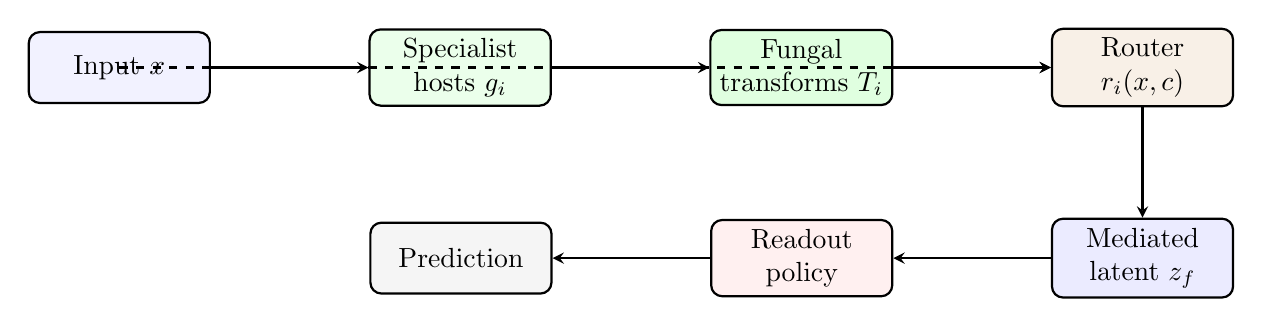
\begin{tikzpicture}[node distance=1.4cm,>=stealth,thick]
\tikzstyle{box}=[draw,rounded corners,minimum width=2.3cm,minimum height=0.9cm,align=center]
\node[box,fill=blue!5] (x) {Input $x$};
\node[box,fill=green!8,right=2.0cm of x] (hosts) {Specialist\\hosts $g_i$};
\node[box,fill=green!12,right=2.0cm of hosts] (trans) {Fungal\\transforms $T_i$};
\node[box,fill=mmalsamber!10,right=2.0cm of trans] (route) {Router\\$r_i(x,c)$};
\node[box,fill=blue!8,below=1.4cm of route] (z) {Mediated\\latent $z_f$};
\node[box,fill=red!6,left=2.0cm of z] (head) {Readout\\policy};
\node[box,fill=gray!8,left=2.0cm of head] (y) {Prediction};
\draw[->] (x) -- (hosts);
\draw[->] (hosts) -- (trans);
\draw[->] (trans) -- (route);
\draw[->] (route) -- (z);
\draw[->] (z) -- (head);
\draw[->] (head) -- (y);
\draw[->,dashed] (x) |- (route);
\end{tikzpicture}
\caption{Conceptual \mmals flow. The route is only part of memory; the mediated latent function and readout behavior also matter.}
\end{figure}

\subsection{Route drift, latent drift, and output drift}

The v0.9 route-function disentanglement introduced three distinct measurements:
\begin{align}
  \Dr &= \mathbb{E}_{x,c}\left[\lVert r_{\mathrm{current}}(x,c) - r_{\mathrm{teacher}}(x,c) \rVert_2^2\right],\\
  \Dz &= \mathbb{E}_{x,c}\left[\lVert z_{f,\mathrm{current}}(x,c) - z_{f,\mathrm{teacher}}(x,c) \rVert_2^2\right],\\
  \Dy &= \mathbb{E}_{x,c}\left[D_{\mathrm{KL}}\left(p_{\mathrm{teacher}}(y|x,c)\,\Vert\,p_{\mathrm{current}}(y|x,c)\right)\right].
\end{align}

A central non-implication is
\begin{equation}
  r_{\mathrm{current}}(x,c) \approx r_{\mathrm{teacher}}(x,c)
  \not\Rightarrow
  z_{f,\mathrm{current}}(x,c) \approx z_{f,\mathrm{teacher}}(x,c).
\end{equation}
Because the route can stay stable while the host or transformation changes, preserving route topology alone is insufficient.

\begin{kidbox}
A bus can take the same road every day, but the passengers can be different. If the passengers are different, the trip has a different meaning. In \mmals, the route is the road, but the useful memory is the passengers plus the destination: what computation actually arrives.
\end{kidbox}

\section{Benchmark setting}

The current main stress benchmark is an overlap-chain class-incremental setting:
\begin{equation}
(0,1) \rightarrow (1,2) \rightarrow (2,3) \rightarrow (3,4) \rightarrow (4,5).
\end{equation}
Labels are global class IDs. This makes the problem harder than disjoint binary task-incremental learning because classes such as 2 and 4 sit at boundaries between contexts. Later notebooks support MNIST, FashionMNIST, RotatedMNIST, and PermutedMNIST.

Runs are staged:
\begin{itemize}[leftmargin=*]
  \item \textbf{smoke}: one seed, small samples, execution and artifact sanity.
  \item \textbf{evidence}: three seeds, larger samples, intermediate scientific signal.
  \item \textbf{robust}: five seeds, same larger samples, stronger qualification.
  \item \textbf{paper}: larger samples and seeds, intended only after the candidate is frozen.
\end{itemize}

\begin{kidbox}
Instead of five separate school quizzes, the teacher makes a chain: quiz 1 has animals 0 and 1, quiz 2 has 1 and 2, quiz 3 has 2 and 3. Now class 2 appears in different neighborhoods. The model must understand the situation, not just memorize the quiz number.
\end{kidbox}

\section{Research chronicle: from v0.1 to v1.1-RC2H}

This section gives the full story in two layers: the PhD-level scientific role and the corresponding explanation for a 12-year-old.

\subsection{v0.1: structural routing toy model}

The first prototype established the basic idea: multiple hosts can be combined by a learned router, and the router can be interpreted as a mycelium-like medium. This was not yet evidence of continual learning. It was an architectural sketch.

\begin{kidbox}
We built the first tiny forest. There were several trees and a mushroom path connecting them. The first question was simple: can the mushroom choose which tree to listen to?
\end{kidbox}

\subsection{v0.2: fairer baselines and capacity checks}

The second step asked whether the apparent benefit was just capacity. The model needed to be compared against simpler neural baselines with comparable or at least explicit parameter counts. This began the discipline that later became central: never compare a mycelium-inspired model only against weak strawmen.

\begin{kidbox}
If one team wins a race with a giant engine and the other team has a bicycle, the race is unfair. v0.2 started checking whether \mmals was winning because of the idea, or just because it had more parts.
\end{kidbox}

\subsection{v0.3: making the fungal medium real}

The fungal medium became more than a metaphor. The architecture began to include specialists, transformations, routes, a mediated latent state, and mutualistic signals. The question became whether a learned medium can stabilize exchanges across hosts.

\begin{kidbox}
The mushroom network stopped being just a drawing. It became a real messenger that could mix advice from different trees.
\end{kidbox}

\subsection{v0.4: warm-up, delayed mutualism, and soft consolidation}

Early training can be fragile. v0.4 introduced warm-up and delayed mutualism so that the system would not over-constrain itself before useful host behavior emerged. The lesson was that mutualism must be timed.

\begin{kidbox}
You should not ask a new team to make perfect teamwork on day one. First everyone learns their job; then the mushroom starts asking them to cooperate.
\end{kidbox}

\subsection{v0.5: route memory and output distillation}

The next hypothesis was that if the router remembers old routing behavior and the outputs remain close to a teacher, old tasks should be preserved. Output distillation gave a behavioral anchor; route memory gave a mechanistic anchor.

\begin{kidbox}
The mushroom tried to remember two things: which path it used before, and what answer the forest gave before. This is like remembering both the road and the final answer.
\end{kidbox}

\subsection{v0.6: route memory under harder benchmarks}

v0.6 asked a causal question: if output distillation is already strong, does route memory add value on harder data? This was the start of a more skeptical style. A mechanism is not accepted because it sounds biologically plausible; it must improve or explain results.

\begin{kidbox}
If remembering the answer already works, does remembering the path help? v0.6 checked whether the path memory was useful or just decorative.
\end{kidbox}

\subsection{v0.7: functional route memory}

v0.7 moved from route preservation toward preserving the computation through routes. This is where the project began to converge on mediated functional memory: the system should preserve the old latent function, not merely the same route probabilities.

\begin{kidbox}
We learned that it is not enough to say, ``I used the same road.'' We must ask, ``Did the road still deliver the same package?''
\end{kidbox}

\subsection{v0.8: final evidence harness}

v0.8 consolidated earlier variants into an evidence harness. It asked which variant performed best and exported results in a more reproducible form. This was the first move from exploratory notebooks to evidence packaging.

\begin{kidbox}
Instead of trying one mushroom trick at a time, v0.8 organized a tournament and wrote down the scores.
\end{kidbox}

\subsection{v0.9: route-function disentanglement}

v0.9 is a major conceptual step. It explicitly distinguishes route drift, functional latent drift, and output drift. It shows that route-only memory can fail badly even when more functional variants remain stable. In the v0.9 scorecard, the route-only control reached about $0.696$ final accuracy with about $0.295$ forgetting, while full functional memory reached about $0.991$ final accuracy and near-zero forgetting.

\begin{table}[h]
\centering
\caption{v0.9 route-function diagnostic summary.}
\begin{tabular}{lrr}
\toprule
Variant & Final accuracy & Forgetting \\
\midrule
Full functional memory & 0.9908 & 0.0004 \\
Distillation only & 0.9913 & 0.0004 \\
Latent only & 0.9905 & 0.0010 \\
Route plus latent & 0.9903 & 0.0011 \\
Route memory only & 0.6959 & 0.2951 \\
\bottomrule
\end{tabular}
\end{table}

The conclusion is not that route information is useless. It is that route information alone is not the memory object. Functional memory must be defined at the level of mediated latent computation and behavior.

\begin{kidbox}
The mushroom remembered the map, but the forest still gave wrong answers. That proved the map alone is not memory. The answer depends on what travels through the map.
\end{kidbox}

\subsection{v0.10: cost and scalability}

v0.10 made the cost question explicit. The model was larger and slower than simple MLP baselines. The scientific trade-off became clear: \mmals must justify its complexity through robustness, auditability, context handling, and functional memory, not just raw accuracy.

\begin{kidbox}
A big forest is expensive to maintain. If it is only a little better than a small garden, maybe it is not worth it. v0.10 asked: what do we get for the extra trees?
\end{kidbox}

\subsection{v0.11: comparative evidence harness}

v0.11 compared \mmals against known continual-learning baselines. In a smoke configuration, full functional memory reached $0.967$ final accuracy and $0.003$ forgetting, behind joint upper bound, PNN, and experience replay, but ahead of LwF, EWC, fine-tuning, and sparse MoE in that run. It used about $1.23$M parameters versus about $218$k for the MLP baselines.

\begin{table}[h]
\centering
\caption{v0.11 comparative smoke result, selected rows.}
\begin{tabular}{lrrrr}
\toprule
Method & Final acc. & Forgetting & Params & Train time (s) \\
\midrule
Joint upper bound & 0.980 & 0.000 & 218k & 1.02 \\
PNN & 0.979 & 0.000 & 218k & 0.37 \\
Experience replay & 0.971 & 0.002 & 218k & 0.49 \\
\mmals full functional memory & 0.967 & 0.003 & 1.23M & 3.99 \\
LwF & 0.962 & 0.003 & 218k & 0.65 \\
EWC & 0.873 & 0.102 & 218k & 0.46 \\
Fine-tuning & 0.821 & 0.142 & 218k & 0.41 \\
Sparse MoE & 0.795 & 0.176 & 1.19M & 1.72 \\
\bottomrule
\end{tabular}
\end{table}

The key lesson was honest: \mmals was not automatically the best on simple benchmarks. Its value proposition must be harder settings, inferred context, auditability, and functional memory.

\begin{kidbox}
The mushroom forest did well, but it did not beat every simpler team. That is okay. It told us the mushroom idea must prove itself on harder races, not just easy ones.
\end{kidbox}

\subsection{v0.12: Hopfield and co-evolution controls}

The Hopfield branch tested whether memory should be understood as a frozen landscape. The evidence suggested that hard frozen-landscape memory is not the main answer. Hopfield-style ideas remain useful as diagnostic controls, but the deployable path remains functional mediated adaptation rather than simply freezing transformations.

\begin{kidbox}
We tried turning part of the forest into stone so it would never change. It remembered some things, but it was not the best way to keep learning. A living forest needs some stable paths and some flexible growth.
\end{kidbox}

\subsection{v0.13 and v0.13.1: co-evolution and warm weak CE}

The co-evolution branch explored transform drift, Jacobian drift, and resistance-like quantities inspired by geometry and physical systems. Warm weak CE ablations showed diagnostic value but did not yet establish a superior training recipe. The research lesson was that geometry can be a microscope before it becomes an optimizer.

\begin{kidbox}
We gave the mushroom a microscope to watch how the paths bend and stretch. The microscope helped us see problems, but it was not yet the best tool to fix them.
\end{kidbox}

\subsection{v0.14 family: inferred context transition}

The major conceptual shift before v1.0 was context inference. Earlier versions were told the task. The v1 direction asks the model to infer the situation from the input and memory, for example through a posterior $q(c|x)$. A small group of examples can be compared with old memory prototypes to infer context.

\begin{kidbox}
Before, someone told the mushroom, ``This is math class.'' Now the mushroom must look around: rulers, triangles, numbers on the board. It has to guess: ``This is probably math class.''
\end{kidbox}

\subsection{v1.0-RC1b: benchmark-ready inferred-context candidate}

v1.0-RC1b consolidated a proto-first \mmals backbone, validation-selected context temperature/blend, and a guarded global head. It made the jump from explicit task IDs toward inferred-context class-incremental stress. The best candidate family became the guarded context-gap policy, often represented as \texttt{paired\_context\_gap\_selected} or \texttt{context\_temp\_blend\_selected\_head\_guard\_035}.

\begin{kidbox}
The mushroom no longer gets a label saying which classroom it entered. It looks at the objects, compares them with old memories, and chooses the path that seems most likely.
\end{kidbox}

\subsection{v1.1-RC2b: strict no-leakage policy selection}

RC2b introduced a strict policy-selection protocol. It trains the same backbone, splits memory into repair, context-selection, and policy-validation partitions, builds candidate policies, scores them on validation memory only, selects before final-test evaluation, and exports audit traces. This is a major methodological improvement.

In the RC2b FashionMNIST robust run, the fixed RC1b context-gap candidate reached $0.9010$ final average accuracy, $0.8183$ min-task accuracy, $0.0556$ forgetting, and $0.8235$ class-2 accuracy. The RC2b automatic selected policy reached $0.8880$ final average accuracy and still beat replay, but failed to match fixed RC1b.

\begin{table}[h]
\centering
\caption{RC2b robust FashionMNIST selected results.}
\begin{tabular}{lrrrrr}
\toprule
Method & Final acc. & Min task & Forgetting & Class 2 & Class 5 \\
\midrule
Fixed RC1b context-gap & 0.9010 & 0.8183 & 0.0556 & 0.8235 & 0.9985 \\
RC2b selected policy & 0.8880 & 0.7773 & 0.0644 & 0.7848 & 0.9985 \\
Experience replay & 0.8390 & 0.6985 & 0.1352 & 0.6188 & 0.9970 \\
\bottomrule
\end{tabular}
\end{table}

\begin{kidbox}
The mushroom made a rule: before looking at the final exam, it chooses its strategy using only practice memories. That is fair. But sometimes it chose the wrong strategy, so the rule was fair but not yet smart enough.
\end{kidbox}

\subsection{RC2c to RC2g: repairing the selector and boundary classes}

RC2c through RC2g were debugging branches:
\begin{itemize}[leftmargin=*]
  \item RC2c added risk-aware penalties, class-2 and min-task floors, no-repair vetoes, and hysteresis.
  \item RC2d aligned the selector to gates and fixed Drive archiving.
  \item RC2e made the selector NaN-safe and improved class-2 behavior.
  \item RC2f protected class 4 after class-4 collapse.
  \item RC2g introduced tri-boundary equilibrium across classes 2, 4, and 5.
\end{itemize}

RC2g smoke looked promising, but RC2g evidence showed the danger of free validation selection. The fixed RC1b context-gap candidate reached about $0.9058$ final accuracy in evidence mode, while RC2g selected about $0.8704$. The selector, not the backbone, was the issue.

\begin{kidbox}
The mushroom kept trying new voting rules. One rule protected class 2 but hurt class 4. Another protected class 4 but hurt class 2. RC2g tried to balance the three difficult children: 2, 4, and 5. It helped, but the mushroom still sometimes picked a worse rule than the old safe one.
\end{kidbox}

\subsection{RC2H: RC1b-anchored conservative selector}

RC2H inverted the selection question. Instead of asking which candidate has the highest proxy score, it asks whether there is enough validation-memory evidence to override the known-good RC1b anchor. It uses the guarded context-gap family as a default deployable anchor and permits overrides only when safety gates are satisfied.

In FashionMNIST evidence mode, RC2H validated the infrastructure but did not yet succeed as a performance selector. The true global guard was best in that run, the RC1b context-gap anchor was second, and RC2H selected policy remained replay-beating but weaker than the best deployable candidate.

\begin{table}[h]
\centering
\caption{RC2H evidence FashionMNIST summary.}
\begin{tabular}{lrrrrr}
\toprule
Method & Final acc. & Min task & Forgetting & Class 2 & Class 5 \\
\midrule
True global guard & 0.8957 & 0.8058 & 0.0623 & 0.8863 & 0.9958 \\
RC1b context-gap anchor & 0.8858 & 0.7908 & 0.0772 & 0.8429 & 0.9958 \\
RC2H selected policy & 0.8788 & 0.7358 & 0.0958 & 0.7696 & 0.9942 \\
Experience replay & 0.8361 & 0.6838 & 0.1415 & 0.6054 & 0.9975 \\
\bottomrule
\end{tabular}
\end{table}

The lesson is that the anchor should likely become a dual safe-anchor family: context-gap plus true global guard. Context-only global candidates should remain audit candidates, not deployment overrides, unless much stronger evidence exists.

\begin{kidbox}
The mushroom learned a safer rule: ``Do not change from the trusted plan unless the new plan is clearly better.'' But two times it still trusted a shortcut that looked good in practice and was weaker on the final test. Next, the mushroom should trust two safe teachers instead of one.
\end{kidbox}

\section{A unified interpretation}

\subsection{What is the memory object?}

The main scientific result of the research program is not a single accuracy number. It is the clarification of the memory object. \mmals memory has at least five layers:
\begin{enumerate}[leftmargin=*]
  \item \textbf{Route memory}: which hosts are weighted.
  \item \textbf{Transformation memory}: how host signals are mapped into exchange space.
  \item \textbf{Latent functional memory}: what mediated representation $\zf$ is computed.
  \item \textbf{Output behavioral memory}: whether predictions remain stable.
  \item \textbf{Context-posterior memory}: whether the system infers the right situation.
\end{enumerate}

A deployment policy adds a sixth layer: the readout/head and its calibration. The RC2 lineage showed that even a strong backbone can be undermined by a weak selector or readout policy.

\begin{kidbox}
Memory is not just ``which road did I take?'' It is the road, the package, the messenger, the final answer, and whether the mushroom understood which village it was visiting.
\end{kidbox}

\subsection{Why the selector became the bottleneck}

RC2b through RC2H show a repeated pattern. The backbone is often capable; diagnostic probes reach high accuracy; fixed guarded policies perform well. But validation-memory policy selection can overfit proxy signals. A policy can look good on validation memory but damage weak boundary classes in final evaluation.

This creates a deployment principle:
\begin{quote}
No-leakage selection is necessary but not sufficient. A selector must also be conservative, anchor-aware, and weak-class aware.
\end{quote}

\begin{kidbox}
Not cheating on the exam is necessary. But even if you do not cheat, you can still choose the wrong study strategy. RC2H is about choosing a strategy carefully, not just fairly.
\end{kidbox}

\section{Cost and engineering interpretation}

\mmals is not free. The v0.11 and RC2 runs make parameter cost visible: MLP baselines are around $218$k parameters, while \mmals variants are around $1.2$M to $1.34$M parameters. The deployment question is therefore not ``does \mmals beat everything on every toy benchmark?'' It is:
\begin{quote}
Does \mmals provide enough robustness, context inference, auditability, and functional-memory control to justify its higher cost in harder continual-learning settings?
\end{quote}

\begin{table}[h]
\centering
\caption{Cost-oriented comparison from selected evidence packages.}
\begin{tabular}{lrrr}
\toprule
Method family & Example final acc. & Params & Model size \\
\midrule
MLP replay baseline & 0.836--0.971 & $\sim$218k & $\sim$0.83 MB \\
PNN baseline & 0.979 in v0.11 smoke & $\sim$218k & $\sim$0.83 MB \\
Sparse MoE & 0.795 in v0.11 smoke & $\sim$1.19M & $\sim$4.54 MB \\
\mmals functional memory & 0.967 in v0.11 smoke & $\sim$1.23M & $\sim$4.70 MB \\
\mmals RC2 family & 0.879--0.901 in harder overlap-chain & $\sim$1.34M & $\sim$5.10 MB \\
\bottomrule
\end{tabular}
\end{table}

\begin{kidbox}
A big forest costs more than a small garden. So the big forest must do something the garden cannot: explain itself, survive harder weather, and remember old paths while growing new ones.
\end{kidbox}

\section{Auditability and Hydro diagnostics}

The v1.1 Hydro branch adds a fluid-inspired diagnostic layer: route drift, latent drift, output drift, adaptive viscosity, Reynolds-like instability, turbulence-like scores, and wave/context entropy. The current conclusion is conservative. Hydro is useful as an audit layer, not yet as the default performance policy.

Hydro metrics matter because they create observability. A model that learns continually should not only output an accuracy number; it should explain whether routes, latent states, outputs, and context posterior were stable or turbulent.

\begin{kidbox}
A river can look calm or turbulent. Hydro gives the mushroom forest a water-meter. It tells us whether the learning flow is smooth or chaotic. For now it is a dashboard, not the steering wheel.
\end{kidbox}

\section{Failure analysis}

The recent selector lineage produced valuable failures.

\subsection{RC2b failure: free strict selection over-selects fragile policies}
RC2b was methodologically correct but not performance-optimal. It selected one policy per checkpoint without final-test leakage, but selected weaker policies too often.

\subsection{RC2e failure: class 2 fixed, class 4 collapsed}
Class-specific rescue can overcorrect. Protecting one boundary class can sacrifice another.

\subsection{RC2f failure: class 4 fixed, class 2 weak again}
Boundary protection must be symmetric and equilibrium-oriented.

\subsection{RC2g failure: tri-boundary balance improves smoke but not evidence}
A selector can pass smoke and still fail evidence. Smoke is execution validation, not scientific validation.

\subsection{RC2H failure: conservative anchor helps but context-only overrides remain unsafe}
Anchoring is necessary, but the safe anchor set should include both context-gap and true global guard. Context-only global candidates should be restricted.

\begin{kidbox}
Every failed version taught us which child fell down: class 2, class 4, class 5, or the selector itself. The failures were not useless. They were like footprints showing where the bridge is weak.
\end{kidbox}

\section{Current best scientific statement}

A careful statement after RC2H is:

\begin{quote}
\mmals has demonstrated a replay-beating, auditable inferred-context continual-learning framework on FashionMNIST overlap-chain experiments. Fixed guarded policies, especially the RC1b context-gap family and the true CE/KL guarded global head, remain stronger than the current automatic selectors. The next deployable selector should be dual-anchor conservative, allowing overrides only from guarded policies with strong validation-memory evidence and weak-class safety gates. Multi-dataset robust qualification remains necessary before stronger claims.
\end{quote}

\begin{kidbox}
The mushroom forest is promising. It beats some simple memory tricks, and it keeps a good notebook of what happened. But it is not ready to drive alone. It still needs a safe rule: trust the strongest known teachers unless a new plan is clearly safer and better.
\end{kidbox}

\section{Next research roadmap}

\subsection{RC2I: dual-anchor conservative selector}

The next notebook should implement a dual-anchor rule:
\begin{itemize}[leftmargin=*]
  \item safe anchors: \texttt{context\_gap\_selected}, \texttt{context\_temp\_blend\_selected\_head\_guard\_035}, and \texttt{proto\_global\_head\_ce\_kl\_guard\_035};
  \item context-only global candidates remain in audit but cannot override by default in evidence/robust;
  \item overrides must be guarded, margin-positive, class-safe, min-task-safe, and forgetting-safe;
  \item report rejection reasons explicitly.
\end{itemize}

\subsection{Multi-dataset robust qualification}

After RC2I passes FashionMNIST evidence and robust, it should be evaluated on:
\begin{enumerate}[leftmargin=*]
  \item MNIST overlap-chain;
  \item FashionMNIST overlap-chain;
  \item RotatedMNIST overlap-chain;
  \item PermutedMNIST overlap-chain.
\end{enumerate}

\subsection{v0.11-style comparative campaign}

The final campaign must include not only accuracy and forgetting but also:
\begin{itemize}[leftmargin=*]
  \item parameters and model size;
  \item training time and memory;
  \item replay buffer items;
  \item min-task and weak-class floors;
  \item context posterior metrics;
  \item Hydro audit metrics;
  \item no-leakage selection traces;
  \item seed-level weak-run diagnosis.
\end{itemize}

\begin{kidbox}
The next big tournament should not only ask who wins. It should ask who wins, who forgets, who is expensive, who explains their decisions, and who stays calm when the game changes.
\end{kidbox}

\section{Limitations}

This research program has important limitations:
\begin{enumerate}[leftmargin=*]
  \item Most claims are still MNIST-family claims.
  \item Smoke runs are not evidence.
  \item Evidence runs are not robust qualification.
  \item The selector remains the main bottleneck.
  \item The model is more expensive than MLP baselines.
  \item Biological inspiration is an analogy, not a biological validation.
  \item No claim of production readiness, safety certification, open-world learning, or industry level qualification is justified yet.
\end{enumerate}

\begin{kidbox}
The mushroom forest has not traveled the whole world yet. It has mostly practiced on small maps. Before we trust it in a real jungle, it needs harder maps, more races, and stricter judges.
\end{kidbox}

\section{Conclusion}

\mmals began as a mycelium-inspired routing architecture and matured into an auditable continual-learning research program. The strongest conceptual contribution is the distinction between route memory and functional memory. The strongest engineering contribution is the evidence harness: no-leakage policy selection, replay comparisons, weak-class diagnostics, context posterior auditing, Hydro stability traces, Drive persistence, manifests, and reproducible packages.

The current state is promising but unfinished. The model has credible replay-beating behavior in the harder overlap-chain setting, but automatic policy selection is not yet reliable enough to be the default deployable mechanism. The next step is not another unconstrained selector. It is a dual-anchor conservative selector followed by multi-dataset robust qualification and a v0.11-style comparative cost/performance campaign.

\begin{kidbox}
The mushroom forest has learned a lot. It can remember, compare, and explain more than before. But the wisest mushroom is not the one that always changes paths. It is the one that knows when to keep the safe path and when a new path is truly better.
\end{kidbox}

\appendix
\section{Milestone table with child-level story}

\begin{longtable}{p{0.13\textwidth}p{0.39\textwidth}p{0.39\textwidth}}
\caption{MMALS research progression.}\\
\toprule
Step & Scientific role & Story for a 12-year-old \\
\midrule
\endfirsthead
\toprule
Step & Scientific role & Story for a 12-year-old \\
\midrule
\endhead
v0.1 & Structural routing toy model. & Build the first mushroom path between smart trees. \\
v0.2 & Fair baselines and capacity checks. & Make sure the mushroom is not winning just because it has a bigger engine. \\
v0.3 & Real fungal medium with hosts and transformations. & The mushroom messenger starts mixing advice from different trees. \\
v0.4 & Warm-up and delayed mutualism. & Let each tree learn its job before forcing teamwork. \\
v0.5 & Route memory and output distillation. & Remember both the road and the answer. \\
v0.6 & Route-memory ablation on harder data. & Check whether remembering the road really helps. \\
v0.7 & Functional route memory. & Check whether the package delivered by the road stayed the same. \\
v0.8 & Evidence harness. & Organize a tournament and record the scores. \\
v0.9 & Route-function disentanglement. & The same road can carry a different package. \\
v0.10 & Cost and scalability. & A big forest must justify its cost. \\
v0.11 & Comparative baselines. & Race the mushroom against known teams. \\
v0.12 & Hopfield/frozen controls. & Test whether turning the forest to stone helps. \\
v0.13 & Geometry and co-evolution diagnostics. & Use a microscope to see how paths stretch. \\
v0.14 & Inferred context. & Guess the classroom without being told the subject. \\
v1.0-RC1b & Proto-first inferred-context candidate with guarded readout. & Choose paths by comparing today with old memories. \\
RC2b & Strict no-leakage policy selection. & Pick a strategy before looking at the final exam. \\
RC2c--RC2g & Risk-aware and boundary-safe selector repairs. & Stop one child from falling without pushing another down. \\
RC2H & RC1b-anchored conservative selector. & Keep the trusted plan unless a new plan clearly wins. \\
RC2I next & Dual-anchor conservative selector. & Trust two safe teachers before accepting a new shortcut. \\
\bottomrule
\end{longtable}

\section{Reproducibility package contents}

The accompanying GitHub-ready package contains:
\begin{itemize}[leftmargin=*]
  \item \texttt{paper/main.tex}: LaTeX source for this article;
  \item \texttt{paper/references.bib}: references;
  \item \texttt{paper/MMALS\_Full\_Story\_PhD\_Article.pdf}: compiled PDF;
  \item \texttt{metrics/}: compact CSV summaries extracted from v0.9, v0.11, RC2b, RC2G, and RC2H evidence packages;
  \item \texttt{notebooks/}: latest RC2H notebook when available;
  \item \texttt{docs/}: selected evidence PDFs;
  \item \texttt{README.md}: GitHub publication instructions.
\end{itemize}

\section{Notation}

\begin{tabular}{ll}
\toprule
Symbol & Meaning \\
\midrule
$x$ & input \\
$c$ & context, explicit in v0.x and inferred in v1 direction \\
$g_i(x)$ & host representation \\
$T_i$ & fungal transformation for host $i$ \\
$r_i(x,c)$ & route weight for host $i$ \\
$z_f(x,c)$ & mediated latent state \\
$D_r$ & route drift \\
$D_z$ & functional latent drift \\
$D_y$ & output drift \\
$q(c|x)$ & inferred context posterior \\
\bottomrule
\end{tabular}


\begin{thebibliography}{99}
\bibitem[Bebber et~al.(2007)]{bebber2007biological} Bebber, D. P., Hynes, J., Darrah, P. R., Boddy, L., and Fricker, M. D. (2007). Biological solutions to transport network design. \emph{Proceedings of the Royal Society B}, 274, 2307--2315.
\bibitem[Bronstein et~al.(2017)]{bronstein2017geometric} Bronstein, M. M., Bruna, J., LeCun, Y., Szlam, A., and Vandergheynst, P. (2017). Geometric deep learning: going beyond Euclidean data. \emph{IEEE Signal Processing Magazine}, 34(4), 18--42.
\bibitem[Chaudhry et~al.(2019)]{chaudhry2019agem} Chaudhry, A., Ranzato, M., Rohrbach, M., and Elhoseiny, M. (2019). Efficient lifelong learning with A-GEM. \emph{ICLR}.
\bibitem[Hopfield(1982)]{hopfield1982} Hopfield, J. J. (1982). Neural networks and physical systems with emergent collective computational abilities. \emph{PNAS}, 79(8), 2554--2558.
\bibitem[Kirkpatrick et~al.(2017)]{kirkpatrick2017ewc} Kirkpatrick, J. et al. (2017). Overcoming catastrophic forgetting in neural networks. \emph{PNAS}.
\bibitem[Li and Hoiem(2017)]{li2017lwf} Li, Z. and Hoiem, D. (2017). Learning without forgetting. \emph{IEEE TPAMI}.
\bibitem[Lopez-Paz and Ranzato(2017)]{lopezpaz2017gem} Lopez-Paz, D. and Ranzato, M. (2017). Gradient episodic memory for continual learning. \emph{NeurIPS}.
\bibitem[Rebuffi et~al.(2017)]{rebuffi2017icarl} Rebuffi, S.-A., Kolesnikov, A., Sperl, G., and Lampert, C. H. (2017). iCaRL: Incremental classifier and representation learning. \emph{CVPR}.
\bibitem[Rusu et~al.(2016)]{rusu2016pnn} Rusu, A. A. et al. (2016). Progressive Neural Networks. \emph{arXiv:1606.04671}.
\bibitem[Simard et~al.(1997)]{simard1997mycorrhizal} Simard, S. W. et al. (1997). Net transfer of carbon between ectomycorrhizal tree species in the field. \emph{Nature}, 388, 579--582.
\bibitem[van de Ven et~al.(2022)]{vandeven2022continual} van de Ven, G. M., Tuytelaars, T., and Tolias, A. S. (2022). Three types of incremental learning. \emph{Nature Machine Intelligence}.
\bibitem[Harbonnier(2026a)]{mmalsv09} Harbonnier, G. (2026a). \emph{MMALS Prototype 0.9: Route-Function Disentanglement and Functional Memory Validation}. Internal research notebook and evidence package.
\bibitem[Harbonnier(2026b)]{mmalsv011} Harbonnier, G. (2026b). \emph{MMALS Prototype 0.11: Comparative Evidence Harness}. Internal research notebook and evidence package.
\bibitem[Harbonnier(2026c)]{mmalsrc2b} Harbonnier, G. (2026c). \emph{MMALS v1.1-RC2b: Strict No-Leakage Policy-Selection Harness}. Internal research notebook and evidence package.
\bibitem[Harbonnier(2026d)]{mmalsrc2h} Harbonnier, G. (2026d). \emph{MMALS v1.1-RC2h: RC1b-Anchored Conservative Selector Harness}. Internal research notebook and evidence package.
\end{thebibliography}


\end{document}
